\documentclass[12pt]{article}
\usepackage[12pt]{moresize}

\usepackage{amsmath}
\usepackage{amssymb}

\usepackage{graphicx}
\usepackage{subcaption}

\usepackage{algorithm}
\usepackage{algpseudocode}
\usepackage{alltt}

\usepackage{multicol}

\usepackage[margin=1in]{geometry}

%\usepackage{hyperref}
%\usepackage[latin1]{inputenc}
%\usepackage{listings}
%\usepackage{scrextend}
%\usepackage{changepage} %Adjustwidth



\title{CprE 489\\Homework 1}
\author{Sean Gordon}
%\date{09/09/2019}

\begin{document}
\maketitle


\hrulefill \\


\noindent 1)\\
\indent (a) Nyquist rate $\Rightarrow$ 2*(22 KHz), and 2$^{10}$ = 1024 levels, $\therefore$ m = 10. \\
\indent \indent Bit Rate = 2(22 KHz) * 10 b/p = 440,000 bps.\\

(b) The levels must be separated by enough voltage so that the noise cannot push the \\
\indent \indent pulse over halfway from one level to another.\\
\indent \indent Thus, the levels must be separated by .2*2 volts.\\

\indent \indent The system can support (1.1V ampl.)*2 / (.2V noise)*2 = 2.2/.4 = 5 levels of logic.\\

\indent (c) Using Shannon Channel Capacity, $C = (12 KHz)*log_2(1+35) = $ 62039.1\\
\indent \indent 150 Kbps $>$ 62039.1, so this rate of transfer is not viable.

\hrulefill \\


\noindent 2)\\
\begin{figure}[h!]
  \centering
  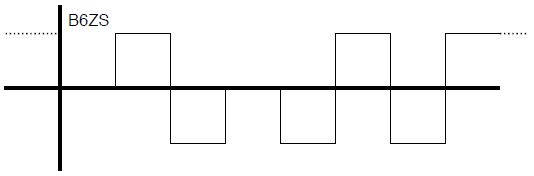
\includegraphics[scale=.8]{B6ZS.JPG}
\end{figure}
\begin{figure}[h!]
  \centering
  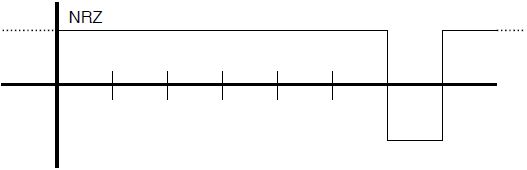
\includegraphics[scale=.8]{NRZI.JPG}
\end{figure}
\begin{figure}[h!]
  \centering
  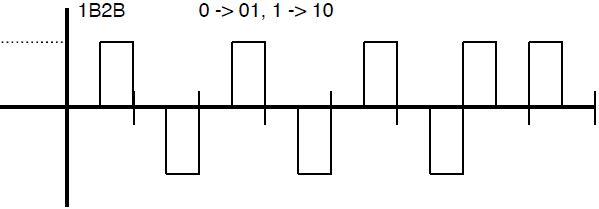
\includegraphics[scale=.8]{1B2B.JPG}
\end{figure}
\begin{figure}[h!]
  \centering
  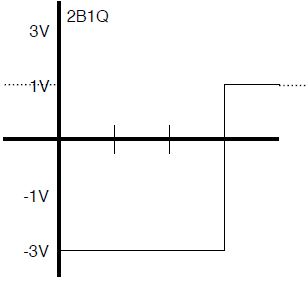
\includegraphics[scale=.8]{2B1Q.JPG}
\end{figure}


\end{document}
















